\section{Plotter}


Advanced graphing cannot be achieved in the transmission domain so the \ds Plotter option allows real-time graphing.
This is a receive only option and a higher level protocol must be adhered to in order to creATE THE GRAPHS. 

\subsection{Protocol}

Initially a command byte is sent followed by as many as $8$ data bytes.
There is a maximum of $4$ bytes for each axis allowing for a range of $2^{32}$ discrete values.
Figure~\ref{fig:cmdByte} and Table~\ref{tab:cmdByte} describes how this byte can control plotting.
Bit $0$, the least significant bit, and bit $1$ remain fixed at logical high.
Bits $2$ and $3$ control plotting where $00$ adds a point, $01$ removes a point and $11$ will erase the whole plot.
The top $4$ bits control the trailing data bytes.

\begin{figure}[h]
   \centering
   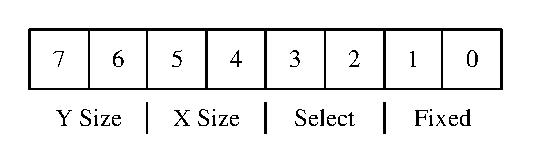
\includegraphics[width=8cm]{cmdByte.pdf}
   \caption{Command byte explained.}
   \label{fig:cmdByte}
\end{figure}

\begin{table}[h]
   \centering
    \begin{tabular}{ | p{3cm} | p{6cm}|p{0.6cm} | p{0.6cm}|}\hline
    \textbf{CMD Byte} 	& \textbf{Function} 						& \textbf{Y}	& \textbf{X}\\ \hline
	00 00 0? 11 			&	Add(0) or Remove(1) point. 				& 1				& 1 						\\ \hline
	00 01 0? 11 			&	Add(0) or Remove(1) point. 				& 1				& 2 						\\ \hline
	00 10 0? 11 			&	Add(0) or Remove(1) point. 				& 1				& 3 						\\ \hline
	00 11 0? 11 			&	Add(0) or Remove(1) point. 				& 1				& 4 						\\ \hline
	01 00 0? 11 			&	Add(0) or Remove(1) point. 				& 2				& 1 						\\ \hline
	01 01 0? 11 			&	Add(0) or Remove(1) point. 				& 2				& 2 						\\ \hline
	01 10 0? 11 			&	Add(0) or Remove(1) point. 				& 2				& 3 						\\ \hline
	01 11 0? 11 			&	Add(0) or Remove(1) point. 				& 2				& 4 						\\ \hline
	10 00 0? 11 			&	Add(0) or Remove(1) point. 				& 3				& 1 						\\ \hline
	10 01 0? 11 			&	Add(0) or Remove(1) point. 				& 3				& 2 						\\ \hline
	10 10 0? 11 			&	Add(0) or Remove(1) point. 				& 3				& 3 						\\ \hline
	10 11 0? 11 			&	Add(0) or Remove(1) point. 				& 3				& 4 						\\ \hline
	11 00 0? 11 			&	Add(0) or Remove(1) point. 				& 4				& 1 						\\ \hline
	11 01 0? 11 			&	Add(0) or Remove(1) point. 				& 4				& 2 						\\ \hline
	11 10 0? 11 			&	Add(0) or Remove(1) point. 				& 4				& 3 						\\ \hline
	11 11 0? 11 			&	Add(0) or Remove(1) point. 				& 4				& 4 						\\ \hline
	xx xx 11 11 			&	Clear entire plot.			 			& 0				& 0 						\\ \hline
    \end{tabular}
    \caption{Command byte options.}
    \label{tab:cmdByte}
\end{table}

The state transition diagram in Figure~\ref{fig:cmdState} explains how the command byte controls the data representation.
A clear command and any other command bytes not listed in Table~\ref{tab:cmdByte} will keep the state machine in the \texttt{CMD} state.
Valid command bytes will move the state machine on the receive data.
First the x-axis data is received followed by the y-axis data.
The first byte in each axis data transmission becomes the most significant byte for that axis.
The three examples in Figure~\ref{fig:cmdExample} explains how the transmission order is used to shift bytes left in the final representation.


\begin{figure}[h]
   \centering
   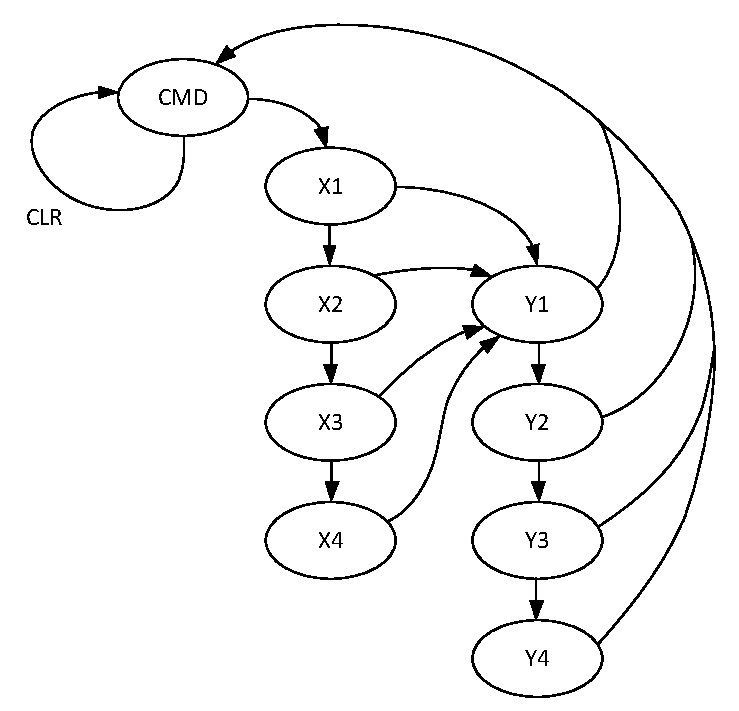
\includegraphics[width=9cm]{stateTransition.pdf}
   \caption{Plotter state transition diagram.}
   \label{fig:cmdState}
\end{figure}


\begin{figure}[h]
   \centering
   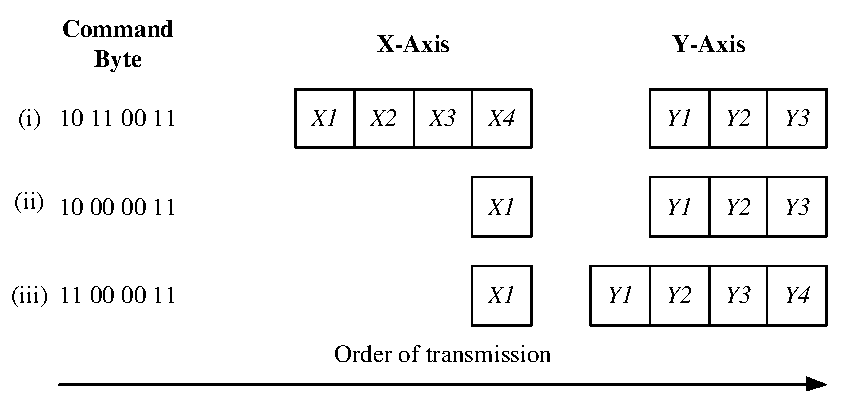
\includegraphics[width=12cm]{cmdExample.pdf}
   \caption{Three example transmissions.}
   \label{fig:cmdExample}
\end{figure}





